\chapter{Background}\label{sec:Background}
- Describe the technical basis of your work \\
- Do not tell a historical story - make it short

\section{PPO}
\marginpar{intro}
In 2017 Schulman et al. introduced the concept of Proximal Policy Optimization (PPO) in
the article ``Proximal Policy Optimization Algorithms''\cite{scwo2017}.
This section is solely based on that article in order to explain the Algorithm.
Policy optimization is the improvement of the action selection strategy $\pi$ based on the
current state $s_{t}$. This is achieved by rotating two steps: 1. sampling data from the policy and 2.
optimizing that data through several epochs.

\marginpar{TRPO, Advantage func}
The origin of PPO lies in a similar approach called Trust Region Policy Optimization (TRPO).
TRPO strives to maximize the following function:
\begin{equation}\label{TRPO}
    \underset{\theta}{maximize}\,\hat{\mathbb{E}}_{t} [\frac{\pi_{\theta}(a_{t} \mid s_{t})}{\pi_{\theta_{old}}(a_{t} \mid s_{t})}
    \hat{A}_{t}-\beta \, KL[\pi_{\theta_{old}}(\cdot \mid s_{t}),\pi_{\theta}(\cdot \mid s_{t})]]
\end{equation}
with $\hat{A}_{t}$ as an estimator of the advantage function. The advantage function often calculated with the
state-value function $V(s)$, a reward $r$ and a discount coefficient $\lambda$ over a period of Time $t$
\begin{equation}\label{advantage}
    \hat{A}_{t} = -V(s_{t})+r_{t}+\lambda r_{t+1}+ \ldots + \lambda^{T-t+1} r_{T-1} + \lambda^{T-t} V(s_{T})
\end{equation}

The fraction in the Minuend of \eqref{TRPO} can be replaced by
$r(\theta)$ %= \frac{\pi_{\theta}(a_{t} \mid s_{t})}{\pi_{\theta_{old}}(a_{t} \mid s_{t})}$
and represents the probability ratio of an
action in the current policy in comparison to the old policy, with $\theta$ being a policy parameter.
The result of $r(\theta)$ is greater than
one, if an action is very probable in the current policy. Otherwise the outcome lies between zero and one.
Schulman et al. further describe that TRPO maximizes the "surrogate" objective
\begin{equation}\label{TRPO surrogate}
    L^{CPI}(\theta) = \hat{\mathbb{E}}_{t}[ \frac{\pi_{\theta}(a_{t} \mid s_{t})}{\pi_{\theta_{old}}(a_{t} \mid s_{t})} \hat{A}_{t}]
    = \hat{\mathbb{E}}_{t}[r(\theta)\hat{A}_{t}]
\end{equation}
However, maximized on its own without a penalty this results in a large outcome and leads to drastic
policy updates.

\marginpar{problem TRPO}
In order to stay in a trust region, as the name suggests, a penalty is subtracted from the
surrogate function \eqref{TRPO surrogate}.
The penalty is the Subtrahend of equation \eqref{TRPO} and contains the fixed coefficient $\beta$.
Regardless of the function details and outcome of $KL$, the coefficient $\beta$
is hard to choose, since different problems require different penalty degrees. Even in a single problem
it could be necessary to adapt the coefficient, due to changes within the setting.

\marginpar{PPO}
Therefore Schulman et al. introduced
\begin{equation}\label{PPO}
    L^{CLIP}(\theta) = \hat{\mathbb{E}}_{t}[\min(r(\theta)\hat{A}_{t},clip(r(\theta), 1-\epsilon, 1+\epsilon)\hat{A}_{t})]
\end{equation}
which is very similar to \eqref{TRPO} but does not require coefficients.
The first part of $\min$ contains $L^{CPI}$ \eqref{TRPO surrogate}.
The second part contains a $clip$ function which narrows the space of policy mutation with
the small hyperparameter $\epsilon$. After applying the clip function $r(\theta)$ lies between
$[1-\epsilon,1+\epsilon]$. Calculating the minimum of the clipped and unclipped probability ratio
produces the lower bound of the unclipped $r(\theta)$, preventing the policy to change drastically.
%[TODO ???]

\marginpar{PPO Algo}
PPO is defined by the following equation
\begin{equation}\label{PPO Algorithm}
    L_{t}^{CLIP+VF+S}(\theta) = \hat{\mathbb{E}}_{t}[L_{t}^{CLIP}(\theta) - c_{1}L_{t}^{VF}(\theta) + c_{2}S[\pi_{\theta}](s_{t})]
\end{equation}
with $c_{1}$ and $c_{2}$ as coefficients. The authors point out that the loss function \\
$L_{t}^{VF} = (V_{\theta}(s_{t})-V_{t}^{targ})^2$
combines the policy surrogate and the value function error term and is
necessary once a neural network shares parameters between policy and value function.
Finally an entropy bonus $S$ is added to ensure exploration.
Schulman et al. continues to show an example of an Algorithm using PPO, see Fig. \ref{fig:ppo_algo_code}.
$N$ detonates (parallel) actors collecting data in T timesteps in each Iteration.
Afterwards the policy is optimized in K epochs by computing the Loss function \eqref{PPO Algorithm} on the
corresponding $NT$ timesteps of data, using a minibatch.
\begin{figure}[hpbt]
    \centering
    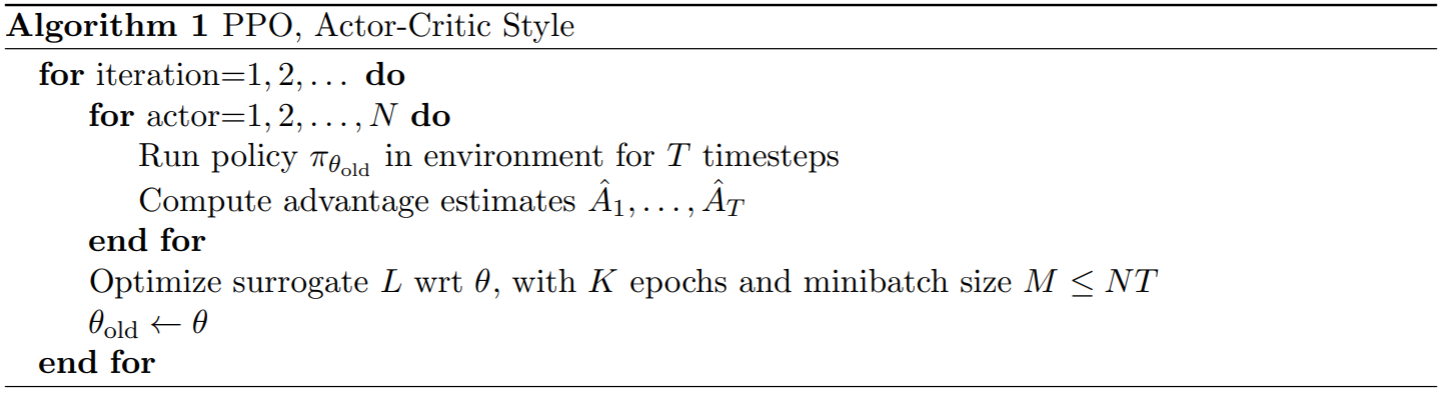
\includegraphics[width=1\textwidth]{pictures/ppo_algo_code.png}\\
    \caption[Exemplary use of PPO]{Exemplary use of PPO, as shown in ``Proximal Policy Optimization Algorithms''\cite{scwo2017}}\label{fig:ppo_algo_code}
\end{figure}

\section{DQN}